
\chapter{Marco Te\'orico}
\section{Introducci\'on}
En esta parte se dar\'an a conocer algunos de los conceptos b\'asico de la Inteligencia Artificial para tener un conocimiento general de lo que ee, ya que es la base de la investigaci\'on de la que posteriormente se hablara.

\section{¿Qu\'e es inteligencia artificial?}

La inteligencia artificial(IA), en una definici\'on amplia y un tanto circular, tiene por objeto el estudio del comportamiento inteligente en las maquinas. A su vez, el comportamiento inteligente supone percibir, razonar, aprender, comunicarse y actuaren entornos complejos. Una de las metas a largo plazo de la IA es el desarrollo de m\'aquinas que puedan hacer todas esas cosas igual, o incluso mejor, que los humanos \citep{Sintesis}.\bigskip

Artificial intelligence (AI) may be defined as the branch of computer science that is concerned with the automation of intelligent behavior \citep{Structures}.\bigskip

Por extra\~no que pueda parecer, lo cierto es que no hay consenso entre los científicos e ingenieros sobre lo que es la inteligencia artificial, y mucho menos se ha llegado a una definici\'on exacta y concisa que nos permita dirimir que programas son o no inteligentes. El problema es que ni siquiera tenemos la certeza de que seamos capaces de definir que es la inteligencia (no artificial) \citep{Fundamentos}. \bigskip

\section{Categor\'ias de la Inteligencia Artificial}

La Inteligencia Artificial se divide en 4 categorías y cada una de ellas es representada con una definición, estas categorías son: \bigskip

\subsection{Sistemas que piensan como humanos}

El nuevo y excitante esfuerzo de hacer que los
computadores piensen... máquinas con mentes, en
el más amplio sentido literal \citep{Haugeland}. \bigskip

\subsection{Sistemas que piensan racionalmente}

El estudio de los c\'alculos que hacen posible
percibir, razonar y actuar \citep{Winston}. \bigskip

\subsection{Sistemas que actúan como humanos}

El arte de desarrollar m\'aquinas con capacidad
para realizar funciones que cuando son realizadas por personas requieren de inteligencia \citep{Kurzweil}. \bigskip

\subsection{Sistemas que actúan racionalmente}

La Inteligencia Computacional es el estudio
del dise\~no de agentes inteligentes \citep{Poole_et}. \bigskip 




\section{Comparaci\'on entre la Inteligencia Natural y Artificial}

En ocasiones, los sistemas de IA resuelven problemas de forma heurística mediante un procedimiento de ensayo y error que incorpora información relevante basada en conocimientos previos. Cuando un mismo problema puede resolverse mediante sistemas naturales (cerebro) o artificiales (computadora), los algoritmos que sigue cada implementación suelen ser completamente diferentes puesto que el conjunto de instrucciones elementales de cada sistema son también diferentes. El cerebro procesa la información mediante la activación coordinada de redes de neuronas en áreas especializadas (cortex visual, cortex motor, etc.). En el sistema nervioso, los datos se transmiten y reciben codificados en variables como la frecuencia de activación de las neuronas o los intervalos en los que se generan los potenciales de acción neuronales. El elevado número de neuronas que intervienen en un proceso de computación natural hace que las fluctuaciones fisiológicas tengan un papel relevante y que los procesos computacionales se realicen de forma estadística mediante la actividad promediada en subconjuntos de neuronas. En un sistema IA, en cambio, las instrucciones básicas son las propias de una computadora, es decir operaciones aritmético-lógicas, de lectura/escritura de registros y de control de flujo secuencial. La tabla 1 describe las diferencias fundamentales entre sistemas de inteligencia artificial y natural en las escalas más relevantes. \bigskip

\begin{table}
	\caption{Comparación entre inteligencia natural y artificial a diferentes niveles } \citep{Benitez}
	\centering
	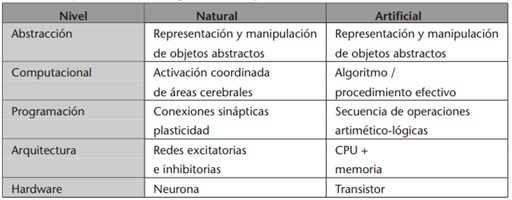
\includegraphics{Img/tabla1.jpg}
\end{table}

La idea principal es que, a pesar de las enormes diferencias entre sistemas naturales y artificiales, a un cierto nivel de abstracción ambos pueden describirse como sistemas de procesado de objetos abstractos mediante un conjunto de reglas. \bigskip


\section{L\'inea del tiempo/historia de la Inteligencia Artificial}

\begin{itemize}
\item 1642-Pascal inventa la primera maquina calculadora me\'anica
\item 1672-Babbage trabaja en calculadoras mec\'anicas programables.
\item 1678-Leibniz: Caracter\'istica Universal.
\item 1842-Babbage: maquina anal\'itica.
\item 1847-Boole: El \'algebra de la l\'ogica. 
\item 1912-Torres Quevedo: Maquina de Ajedrez.
\item 1936-Turing: Maquina Universal.
\item 1942-Asimov publica sus famosas tres leyes de la rob\'otica.
\item 1945-Eckert y Mauchley: ENIAC.
\item 1948-Wiener: Cibern\'etica.
\item 1950-Shannon: Programa que juega ajedrez.
\item 1950-Turing: juego de imitaci\'on.
\item 1950-Turing propone un test para comprobar el desarrollo inteligente de una  maquina.
\item 1959-Rosenblatt: Perceptron.
\item 1965-Zadeh: L\'ogica difusa.
\item 1971-HERSAY I: Reconocimiento del habla.
\item 1972-Kowalski: Programaci\'on Lógica.
\item 1982-Hopfield: Redes Neuronales.
\item 2000-Mascotas Robots disponibles en el mercado. 
\item 2007-Masssimo Verassola y Boris Schraiman: La inteligencia artificial aprende a rastrear olores como los insectos.
\item 2009-ASIMO es capaz de ser controlado por una persona mediante un dispositivo ICC con un 90.6\% de aciertos.
\end{itemize}

\section{Inteligencia Artificial convencional y computacional}

\cite{convencional_computaciona} afirma que la IA se divide en dos escuelas de pensamiento, estas son la inteligencia artificial y la inteligencia computacional como se muestra a continuaci\'on.

\subsection{INTELIGENCIA ARTIFICIAL CONVENCIONAL} 

También conocido como IA simbólico-deductiva e IA débil. Está basada en el análisis formal y estadístico del conocimiento humano ante diferentes problemas: \bigskip 

\begin{itemize}
\item Razonamiento basado en casos: Ayuda a tomar decisiones mientras se resuelven ciertos problemas concretos.

\item Sistemas expertos: Infieren una solución a través del conocimiento previo del contexto en que se aplica y de ciertas reglas o relaciones.

\item Redes bayesianas: propone soluciones mediante inferencia estadística.

\item Inteligencia artificial basada en comportamientos: sistemas complejos que tienen autonomía y pueden auto-regularse y controlarse para mejorar
\end{itemize}

\subsection{INTELIGENCIA ARTIFICIAL COMPUTACIONAL} 

También conocida como IA subsimbólica-inductiva e IA fuerte; implica desarrollo o aprendizaje iterativo, por ejemplo, modificaciones interactivas de los parámetros en sistemas conexionistas. El aprendizaje se realiza basándose en datos empíricos. Algunos métodos de esta rama incluyen: \bigskip

\begin{itemize}
\item Máquina de vectores soporte: Sistemas que permiten reconocimiento de patrones genéricos de gran potencia.

\item Redes neuronales: sistemas con grandes capacidades de reconocimiento de patrones.

\item Modelos ocultos de Markov: Aprendizaje basado en dependencia temporal de eventos probabilísticas.

\item sistemas difusos: Técnicas para lograr el razonamiento bajo incertidumbre. Ha sido ampliamente usada en la industria moderna y en productos de consumo masivo, como las lavadoras.

\item Computación evolutiva: aplica conceptos inspirados en la biología, tales como población, mutación y supervivencia del más apto para generar soluciones sucesivamente mejores para un problema.
\end{itemize}

\section{\'Ambitos de aplicaci\'on de la Inteligencia artificial}

La inteligencia artificial combina varios campos, como la rob\'otica, los sistemas expertos y otros, los cuales tienen un mismo objetivo, que es tratar de crear m\'aquinas que puedan pensar por s\'i solas, lo que origina que hasta la fecha existan varios estudios y aplicaciones, dentro de las que se encuentran las redes neuronales, el control de procesos o los algoritmos gen\'eticos \citep{ambitos}.

\subsection{La AI en la rob\'otica}

Los robots son dispositivos compuestos de censores que reciben datos de entrada que manda una computadora, la cual ordena al robot que efect\'ue una determinada acci\'on.

Hoy en d\'ia, una de las finalidades de la construcci\'on de robots es su intervenci\'on con rapidez, calidad y precisi\'on en los procesos de fabricaci\'on encargados de realizar trabajos repetitivos en la fabricaci\'on.

\subsection{\'Areas de aplicaci\'on de la IA}

Pero tambi\'en hay \'areas de aplicaci\'on. En efecto, estos procesos de la AI se aplican en los sistemas reales en una gran variedad de ramas y problemas:

\begin{itemize}
\item Gesti\'on y control: an\'alisis inteligente, fijaci\'on de objetivos.
\item Fabricaci\'on: dise\~no, planificaci\'on, programac\'on, monitorizaci\'on, control, gesti\'on de proyectos, rob\'otica simplificada y visi\'on computarizada.
\item Educaci\'on: adiestramiento práctico, ex\'amenes y diagn\'ostico.
\item Ingenier\'ia: dise\~no, control y an\'alisis.
\item Equipamiento: dise\~no, diagn\'ostico, adiestramiento, mantenimiento, configuraci\'on, monitorizaci\'on y ventas.
\item Cartograf\'ia: interpretaci\'on de fotograf\'ias, dise\~no, resoluci\'on de problemas cartogr\'aficos.
\item Profesiones: abogac\'ia, medicina, contabilidad, geología, qu\'imica.
\item Software: ense\~nanza, especificaci\'on, diseño, verificaci\'on, mantenimiento.
\item Sistemas de armamento: guerra electr\'onica, identificaci\'on de objetivos, control adaptativo, proceso de im\'agenes, proceso de s\~nales.
\item Proceso de datos: educaci\'on, interface en lenguaje natural, acceso inteligente a datos y gestores de bases de datos, an\'alisis inteligente de datos.
\item Finanzas: planificaci\'on, an\'alisis, consultor\'ia. 
\end{itemize}

\subsection{Aplicaciones comerciales de la inteligencia artificial}

Pero también la AI tiene numerosas aplicaciones comerciales en el mundo de hoy. V\'aase:

\begin{itemize}
\item Configuraci\'on: selecci\'on de distribuci\'on de los componentes de un sistema de computaci\'on.
\item Diagnosis: hardware inform\'atico, redes de ordenadores, equipos mec\'anicos, problemas m\'edicos, aver\'ias telef\'onicas, instrumentaci\'on electr\'onica, circuitos electr\'onicos, aver\'ias automovil\'isticas.
\item Interpretaci\'on y an\'alisis: datos geol\'ogicos para prospecci\'on petrolífera, compuestos qu\'imicos, an\'alisis de se\~nales, problemas matem\'aticos complejos, evaluaci\'on de amenazas militares, an\'alisis de circuitos electr\'onicos, datos biol\'ogicos (coronarios, cerebrales y respiratorios), informaci\'on de radar, sonar e infrarrojos.
\item Monitorizaci\'on: equipos, monitorizaci\'on de procesos, fabricaci\'on y gesti\'on de procesos cient\'ificos, amenazas militares, funciones vitales de pacientes hospitalizados, datos financieros en tiras de papel perforado por tele impresora, informes industriales y gubernamentales.
\item Planificaci\'on: gesti\'on de activo y pasivo, gesti\'on de cartera, análisis de cr\'editos y pr\'estamos, contratos, programaci\'on de trabajos de taller, gesti\'on de proyectos, planificaci\'on de experimentos, producci\'on de tarjetas de circuito impreso.
\item Interfaces inteligentes: hardware (fiscal) de instrumentaci\'on, programas de computadora, bases de datos m\'ultiples, paneles de control.
\item Sistemas de lenguaje natural: interfaces con bases de datos en lenguaje natural, gesti\'on de impuestos (ayudas para contabilidad), consultoría en temas legales, planificaci\'on de fincas, consultor\'ia de sistemas bancarios.
\item Sistemas de dise\~no: integraci\'on de microcircuitos en muy alta escala, síntesis de circuitos electr\'onicos, plantas qu\'imicas, edificios, puentes y presas, sistemas de transporte.
\item Sistemas de visión computarizada: selecci\'on de piezas y componentes, ensamblado, control de calidad.
\item Desarrollo de software: programaci\'on autom\'atica.
\end{itemize}



